\section{Evaluation}
\label{sec:evaluation}
\emergencystretch=2em

The gateway of Section~\ref{sec:system} is trained on whole, synthetically wrapped strings, scores four request contexts on average at serving time, and blocks at a threshold that was set by hand. A claim that federating such a classifier helps therefore has to survive three changes of protocol: from the controlled design to the shipped model, from random to grouped splits, and from the training view of a request to the serving view. The central question is when federation across sites with different benign profiles or attack mixes improves the classifier, at what cost, and where the security limit of the aggregation lies. Every number below comes from a committed result file, named in Table~\ref{tab:eval-pipelines} or in the caption of the table or figure that reports it; a number without such a source is labelled as an earlier measurement.

\subsection{Data and Protocols}
\label{sec:eval-setup}

\paragraph{Public corpus strings.}
The attack strings are entries of the public SecLists corpus~\cite{seclists}: SQL injection (SQLi, 17 lists) and cross-site scripting (XSS, 7 lists). Benign strings are path tokens and endpoint names from the same corpus, in two profiles: ``web'' (\texttt{raft-small-words}) and ``API'' (\texttt{api-seen-in-wild}, \texttt{api-endpoints}, \texttt{graphql}). None of this is captured production traffic. Training examples are additionally wrapped in synthetic request contexts (below), and the one external benchmark we use, CSIC~2010 (Section~\ref{sec:eval-real}), is an academically generated HTTP dataset, not a site's log. Table~\ref{tab:eval-corpora} lists the deduplicated corpora.

\begin{table}[t]
\centering
\caption{Unique corpus strings after deduplication and the exact-string 70/30 split used by the shipped-model study (\texttt{fed\_model.json}).}
\label{tab:eval-corpora}
\begin{tabular}{@{}lrrr@{}}
\toprule
\textbf{Class} & \textbf{Unique} & \textbf{Train} & \textbf{Test} \\ \midrule
Benign (web) & 43{,}007 & 30{,}104 & 12{,}903 \\
Benign (API) & 8{,}013 & 5{,}609 & 2{,}404 \\
SQLi & 681 & 476 & 205 \\
XSS & 523 & 366 & 157 \\ \bottomrule
\end{tabular}
\end{table}

\paragraph{Splits and wrappers.}
Drawing train and test sets independently from a pool of a few hundred attack strings puts identical strings on both sides and measures memorisation, so the first protocol splits by unique string. An earlier configuration in which benign and attack requests used different templates let a classifier reach a perfect ROC-AUC on attack classes it never trained on, by separating URL shapes; benign and malicious values now share the same request context. The early gateway models also learned payload length: corpus attacks are short, so benign requests carrying headers, JSON or prose were flagged. \texttt{train\_production\_model.py} therefore wraps every sample in one of seven contexts drawn uniformly (the bare value; a user-agent prefix; a cookie header; a full URL with query string; a JSON body with a prose field; a form body with a CSRF token; a prose sentence before the value). The wrappers shifted the intercept to $b\approx-5.57$ and led to the deployed $\tau=0.15$ (\texttt{BLOCK\_THRESHOLD} in \texttt{continuous\_waf.py}). Unique-string splitting does not remove near-duplicates, since the sqlmap and fuzzdb lists contain many variants of one template; the grouped splits of Section~\ref{sec:eval-deployed} address this.

\paragraph{Nodes, features and training.}
Each node trains on 3{,}000 benign and 1{,}000 attack samples. In the \emph{attack} axis the nodes share a benign profile and see different attack mixes; in the \emph{domain} axis both see the full attack mix, node~A web paths and node~B API endpoints. \emph{Syntactic} features are three scalars (length, non-alphanumeric count, Shannon entropy) scaled by fixed constants; \emph{$n$-gram} features are $\ell_2$-normalised hashed character 3-gram counts in $D$ buckets plus the three scalars, giving dimension $D+3$. The classifier is logistic regression trained by SGD (log loss, $\ell_2$ penalty $10^{-4}$, constant step $0.01$). Offline FedAvg runs $R=20$ rounds of $E=30$ local epochs with sample-weighted averaging; isolated baselines train for $R\cdot E$ epochs. The online aggregation of the deployed cloud server is a coordinate-wise median, evaluated separately in Section~\ref{sec:eval-byzantine}.

\paragraph{Metrics and operating points.}
ROC-AUC and PR-AUC are threshold-free. Recall is reported either at a pooled false-positive budget (0.1\% or 1\%) or at a fixed probability threshold, and every table and figure below names which. The threshold~0.5 is the convention of the controlled studies; $\tau=0.15$ is the deployed value.

\begin{table*}[t]
\centering
\caption{The four evaluation pipelines. Their data, splits and operating points differ and their numbers are not interchangeable.}
\label{tab:eval-pipelines}
\footnotesize
\setlength{\tabcolsep}{4pt}
\begin{tabular}{@{}p{4.0cm}p{3.0cm}p{3.0cm}p{0.9cm}p{2.2cm}p{2.8cm}@{}}
\toprule
\textbf{Result file} & \textbf{Model} & \textbf{Split} & \textbf{Seeds} & \textbf{Scored unit} & \textbf{Operating point} \\ \midrule
\texttt{matrix\_\allowbreak results.json} & $D{=}64$, unaugmented & exact-unique & 8 & whole string & 0.1\% FPR, $0.5$ \\
\texttt{fed\_model.json} & shipped $D{=}256$, augmented & exact-unique & 8 & whole string & 0.1\% FPR, $0.5$ \\
\texttt{eval\_deployed\_\allowbreak results.json} & recipe retrained & random / cluster / source & 20 & whole and gateway & 1\%, 0.1\% (validation), $0.15$ \\
\texttt{real\_data\_\allowbreak results.json} & shipped; pooled retrain (LOCO) & CSIC; leave-one-corpus-out & 1; 3 & gateway contexts & $0.5$, $0.15$ \\ \bottomrule
\end{tabular}
\end{table*}

\subsection{Which Heterogeneity Axis Does Federation Exploit?}
\label{sec:eval-matrix}

The first question is the controlled one: with two nodes, does federated averaging help more when the nodes differ in attack mix or in benign profile? Table~\ref{tab:eval-matrix} crosses both axes with both feature sets at $D=64$ (\texttt{fl\_simulation\_v4.py}).

\begin{table*}[t]
\centering
\caption{Controlled matrix, unaugmented $D{=}64$ configuration (\texttt{matrix\_results.json}; mean over eight seeds, standard deviation of ROC-AUC in parentheses). Recall at 0.1\% pooled FPR; FPR-API at threshold 0.5. Bold: best ROC-AUC per feature set and axis; differences below 0.0005 are treated as ties.}
\label{tab:eval-matrix}
\begin{tabular}{@{}llrrrr@{}}
\toprule
\textbf{Features} & \textbf{Axis / model} & \textbf{ROC-AUC} & \textbf{XSS} & \textbf{SQLi} & \textbf{FPR-API} \\ \midrule
\multirow{6}{*}{Syntactic (3)}
 & attack: Edge A & 0.9723 (0.0055) & 0.894 & 0.679 & 0.0140 \\
 & attack: Edge B & \textbf{0.9891} (0.0034) & 0.922 & 0.777 & 0.0123 \\
 & attack: Federated & 0.9788 (0.0050) & 0.903 & 0.737 & 0.0080 \\
 & domain: Edge A & 0.9803 (0.0054) & 0.902 & 0.736 & 0.0085 \\
 & domain: Edge B & \textbf{0.9919} (0.0033) & 0.946 & 0.841 & 0.0010 \\
 & domain: Federated & 0.9902 (0.0034) & 0.926 & 0.809 & 0.0012 \\ \midrule
\multirow{6}{*}{$n$-gram, $D{=}64$ (67)}
 & attack: Edge A & 0.9532 (0.0056) & 0.904 & 0.581 & 0.0135 \\
 & attack: Edge B & \textbf{0.9895} (0.0031) & 0.913 & 0.805 & 0.0098 \\
 & attack: Federated & 0.9826 (0.0044) & 0.927 & 0.764 & 0.0053 \\
 & domain: Edge A & 0.9839 (0.0043) & 0.915 & 0.768 & 0.0102 \\
 & domain: Edge B & \textbf{0.9916} (0.0035) & 0.954 & 0.850 & 0.0013 \\
 & domain: Federated & \textbf{0.9918} (0.0032) & 0.952 & 0.833 & 0.0010 \\ \bottomrule
\end{tabular}
\end{table*}

On the attack axis each silo is blind to the other's attack class, and federation recovers most of the gap for the weaker node: with $n$-grams, Edge~A's SQLi recall rises from 0.581 to 0.764. It stays below Edge~B (0.805), the outcome expected when local optima diverge~\cite{li2020convergence} and the average falls between them. On the domain axis the federated model ties the better silo in ROC-AUC (0.9918 against 0.9916, with a seed standard deviation of 0.003) and trails it on SQLi recall (0.833 against 0.850). What federation buys there is the better silo's behaviour on both benign domains without knowing in advance which silo that is: Edge~A alone has a 1.0\% API false-positive rate at threshold 0.5, and the federated model brings it to 0.10\%. In this matrix, then, federation lifts the weaker node and lowers cross-domain false positives; it does not exceed the best isolated model. Whether that survives augmentation is the next test.

\subsection{Does the Result Survive Augmentation?}
\label{sec:eval-detection}

Table~\ref{tab:eval-detection} repeats the domain-split comparison for the shipped configuration ($D=256$, augmented), still with exact-unique splits and whole-string scoring.

\begin{table}[t]
\centering
\caption{Shipped $D{=}256$ augmented model, domain-split nodes, exact-unique split, whole-string scoring (\texttt{fed\_model.json}); mean $\pm$ std over eight seeds. Recall at 0.1\% pooled FPR; FPR at threshold 0.5, not at the deployed 0.15.}
\label{tab:eval-detection}
\resizebox{\columnwidth}{!}{%
\begin{tabular}{@{}lrrrrrr@{}}
\toprule
\textbf{Model} & \textbf{ROC-AUC} & \textbf{PR-AUC} & \textbf{XSS} & \textbf{SQLi} & \textbf{FPR web} & \textbf{FPR API} \\ \midrule
Edge A & 0.9859$\pm$0.0035 & 0.9871$\pm$0.0032 & 0.954$\pm$0.046 & 0.807$\pm$0.073 & 0.0010 & 0.0052 \\
Edge B & 0.9938$\pm$0.0036 & 0.9940$\pm$0.0031 & 0.979$\pm$0.020 & \textbf{0.879}$\pm$0.033 & 0.0008 & 0.0005 \\
Federated & \textbf{0.9947}$\pm$0.0019 & \textbf{0.9950}$\pm$0.0017 & \textbf{0.980}$\pm$0.022 & 0.865$\pm$0.059 & 0.0005 & 0.0007 \\ \bottomrule
\end{tabular}}
\end{table}

The federated model has the highest mean ROC-AUC and the smallest seed variance, but its margin over Edge~B (0.0009) is a fraction of one standard deviation: it exceeds Edge~B in 5 of 8 seeds and Edge~A in 8 of 8. On SQLi recall, the hardest class, Edge~B is higher on average (0.879 against 0.865) and the federated model falls 0.09 short in the worst seed. The reading is the same as in the matrix. The federated model matches the better silo, beats the silo trained on the wrong benign domain, and has the lowest web false-positive rate. Over the 20 rounds, global ROC-AUC (last seed) is 0.9872 after round~1, 0.9943 after round~3 and 0.9958 after round~20, so most of the offline gain arrives within three rounds; this trajectory says nothing about how fast a pattern would propagate through the deployed 15\,s synchronisation. We do not report a hashing-dimension sweep: the only curve in the repository was hard-coded in \texttt{make\_figures.py} from a pre-augmentation run and cannot be regenerated from a result file.

Two things in this protocol favour every model. The test strings are exact-unique but not near-unique, and the threshold of 0.5 is not the one the gateway uses.

\subsection{Deployed Operating Point and Serving View}
\label{sec:eval-deployed}

\texttt{eval\_deployed.py} asks what happens when both are corrected. It retrains the production recipe (D=256 3-gram, domain split, FedAvg $R{=}20$, $E{=}30$, same wrappers) on 60/20/20 train/validation/test splits, adds a pooled model trained on all data as the missing centralised baseline, selects thresholds on validation only, and repeats everything for 20 seeds with a fresh split each time. Three split modes control leakage: \emph{random} (exact-unique, as above), \emph{cluster} (near-duplicate groups kept together) and \emph{source} (whole SecLists files held out for the attack classes). The share of test attack payloads with a train payload at normalised Levenshtein similarity of at least 0.8 is 76\% (SQLi) and 34\% (XSS) under random splitting, 0 under cluster splitting and 27\% and 13\% under source splitting. We use the cluster split as the primary protocol. The shipped \texttt{fed\_model.json} is not scored here, because its training payloads overlap any random test split: the results characterise the recipe, and the 0.15 threshold they test was chosen for the shipped weights.

Each test payload is evaluated in two views. In the \emph{whole} view the wrapped string is scored once, as in training. In the \emph{gateway} view the payload is placed in one of six request locations with benign background headers, then path, query, \texttt{User-Agent}, \texttt{Referer}, \texttt{Cookie} and body are scored separately and the maximum is taken, which reproduces \texttt{continuous\_waf.py}; the request averages 4.0 scored contexts. A third view scores only the injected context and isolates the effect of the maximum from that of the request mix. The benign background and the request construction are synthetic, and the benign strings remain word lists.

\begin{table*}[t]
\centering
\caption{Retrained recipe at the deployed threshold $\tau=0.15$, cluster split, 20 seeds, mean (95\% $t$-interval over seeds) (\texttt{eval\_deployed\_results.json}). FPR is over pooled web and API benign test strings; recall is over every unique test attack payload with three wrappers each. ``Whole'': one wrapped string; ``gateway'': per-context scoring with maximum.}
\label{tab:eval-deployed}
\begin{tabular}{@{}lcccccc@{}}
\toprule
 & \multicolumn{2}{c}{\textbf{ROC-AUC}} & \multicolumn{2}{c}{\textbf{FPR at 0.15}} & \multicolumn{2}{c}{\textbf{SQLi recall at 0.15}} \\
\textbf{Model} & whole & gateway & whole & gateway & whole & gateway \\ \midrule
Edge A (web) & .949 (.940--.959) & .929 (.916--.941) & .155 & .169 & .834 & .797 \\
Edge B (API) & .960 (.953--.967) & .894 (.880--.909) & .182 & .679 & .880 & .933 \\
Federated & .959 (.951--.967) & .921 (.908--.934) & .114 & .349 & .848 & .852 \\
Pooled & .959 (.951--.967) & .922 (.909--.935) & .097 & .278 & .842 & .829 \\ \bottomrule
\end{tabular}
\end{table*}

\begin{figure}[t]
\centering
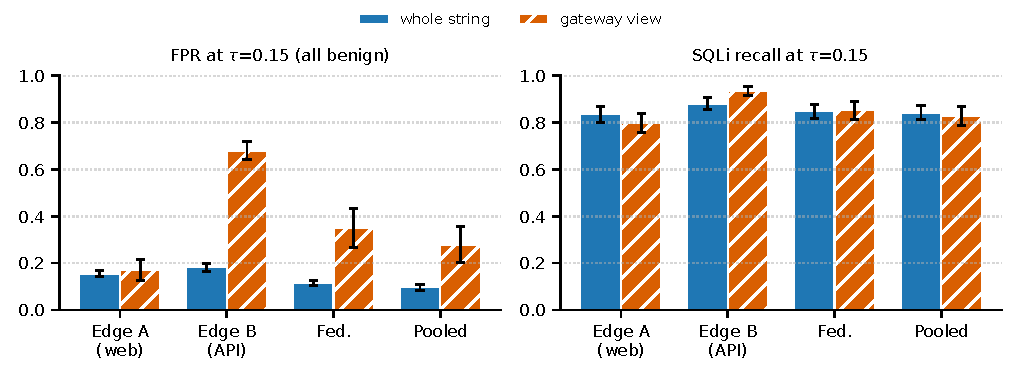
\includegraphics[width=\columnwidth]{figures/fig_deployed.pdf}
\caption{False-positive rate and SQLi recall at $\tau=0.15$ for the retrained recipe, cluster split, 20 seeds, 95\% intervals (\texttt{eval\_deployed\_results.json}). The whole-string and gateway views score the same payloads; only the gateway view takes the maximum over request contexts.}
\label{fig:eval-deployed}
\end{figure}

\paragraph{Ranking in the whole view.}
With grouped splits the three trained models are close and below their exact-unique values: federated ROC-AUC is 0.959 on the cluster split and 0.967 on the random split. Table~\ref{tab:eval-paired} gives the paired differences. Against the silo that validation selects (Edge~B in 15 of 20 cluster seeds) the federated AUC gain is $+0.0021$ with an interval that contains zero; against the silo that turns out best on test it is $-0.0019$ ($-0.0032$ to $-0.0006$); against the pooled model it is $+0.0003$ (interval containing zero) in the cluster mode. Federation matches centralised training in AUC and in recall at the validation-selected 1\% FPR (SQLi difference $0.000$), which is the benchmark the earlier studies lacked: on this data federation gives up nothing to pooling, and gains nothing over it either. Against the selected silo it improves SQLi and XSS recall at 1\% FPR by 0.013 to 0.025 in every split mode, and lowers false positives at $\tau=0.15$ by 0.037 to 0.069 absolute. The one place where the federated model is measurably worse than the alternative is against pooling at the deployed threshold: its FPR is higher by 0.017 (0.003 to 0.032) on the cluster split.

\begin{table*}[t]
\centering
\caption{Federated minus baseline, paired over 20 seeds, whole-string view, with 95\% intervals (\texttt{eval\_deployed\_results.json}). ``Selected silo'' is chosen by validation ROC-AUC; ``best silo'' is the test-optimal one and is optimistic for the silo. Recall at the validation-selected 1\% FPR threshold; FPR at $\tau=0.15$.}
\label{tab:eval-paired}
\begin{tabular}{@{}lccccc@{}}
\toprule
\textbf{Split} & \textbf{AUC vs.\ selected} & \textbf{AUC vs.\ best} & \textbf{AUC vs.\ pooled} & \textbf{SQLi vs.\ selected} & \textbf{FPR vs.\ selected} \\ \midrule
random & $-.0004$ ($-.0014$, $+.0007$) & $-.0004$ ($-.0014$, $+.0006$) & $+.0002$ ($.0000$, $+.0003$) & $+.025$ ($+.017$, $+.033$) & $-.069$ \\
cluster & $+.0021$ ($-.0013$, $+.0055$) & $-.0019$ ($-.0032$, $-.0006$) & $+.0003$ ($-.0001$, $+.0006$) & $+.024$ ($+.015$, $+.033$) & $-.056$ \\
source & $+.0041$ ($+.0011$, $+.0070$) & $-.0004$ ($-.0025$, $+.0017$) & $.0000$ ($-.0003$, $+.0003$) & $+.020$ ($+.007$, $+.033$) & $-.037$ \\ \bottomrule
\end{tabular}
\end{table*}

\paragraph{The deployed threshold.}
The deployed value is not a conservative one. At $\tau=0.15$ the federated recipe flags 11.4\% of benign whole strings (cluster split; interval 10.3--12.5\%), where the validation-selected 1\% budget would flag 1.0\%. In exchange it recovers SQLi recall of 0.848 against 0.766 at the 1\% budget. Because every benign string is a path token, an 11\% rate is not an estimate of production behaviour; the CSIC result below suggests it is a lower bound.

\paragraph{The serving view.}
Scoring by context changes the ranking. Federated AUC falls from 0.959 to 0.921; the FPR at $\tau=0.15$ rises from 0.114 to 0.349 (interval 0.267--0.432), and Edge~B, trained only on API strings, goes from 0.182 to 0.679. The injected-context-only view gives 0.052 for the federated model, so the benign background headers account for most of the excess: the maximum over about four contexts exposes any context that the model scores high on every benign request. In this view the federated model has a higher gateway AUC than the silo selected on validation ($+0.017$, 15 of 20 seeds) only because validation tends to pick Edge~B, the silo that degrades most; Edge~A alone has gateway AUC 0.929 against 0.921 federated. The pooled model is better than the federated one in this view by 0.0009 ($-0.0014$ to $-0.0003$ for federated minus pooled). Which silo a site would have trained, and which view it serves, decide whether federation looks like a gain. A synthetic benign background already produces a 35\% false-positive rate at the deployed threshold; the next question is what a real one produces.

\subsection{Real Data: A Deployment Failure}
\label{sec:eval-real}

\subsubsection*{CSIC 2010 through the gateway scorer}


\texttt{real\_data\_eval.py} scores CSIC~2010 requests with the shipped \texttt{fed\_model.json} through the same context extraction as the gateway. The corpus has 72{,}000 normal requests (the training and test files pooled, 36{,}000 each) and 25{,}065 anomalous ones; the files are fetched from a public mirror, and their SHA-256 digests are recorded in the result file. No CSIC string was used in training. The anomalous class mixes all attack types in the dataset (SQLi, XSS, buffer overflow, CRLF injection, path traversal, information gathering, parameter tampering) and carries no sub-type label, so recall on it is not attack-family recall.

\begin{table}[t]
\centering
\caption{CSIC 2010 through the gateway scorer with the shipped model (\texttt{real\_data\_results.json}); fraction of requests flagged at $\tau=0.15$. ``All contexts'': maximum over path, query, \texttt{User-Agent}, cookie and body, as deployed. ``Payload only'': query and body. Last column: normal requests at threshold~0.5. Counts: 72{,}000 normal, 25{,}065 anomalous.}
\label{tab:eval-csic}
\small
\begin{tabular}{@{}lrrr@{}}
\toprule
\textbf{Scorer} & \textbf{Normal} & \textbf{Anomal.} & \textbf{Normal, 0.5} \\ \midrule
All contexts (gateway) & 1.000 & 1.000 & 1.000 \\
Payload only & 0.191 & 0.523 & 0.167 \\ \bottomrule
\end{tabular}
\end{table}

\begin{figure}[t]
\centering
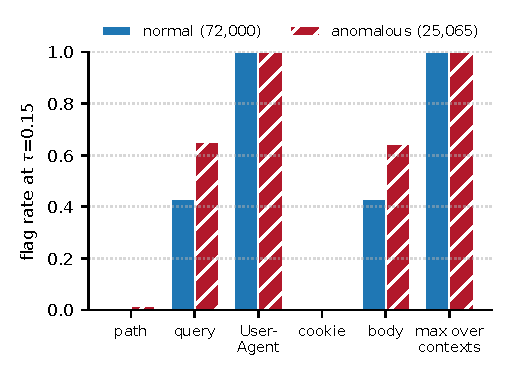
\includegraphics[width=0.85\columnwidth]{figures/fig_csic.pdf}
\caption{Fraction of CSIC~2010 requests whose context scores at least $\tau=0.15$, by context and for the gateway maximum, shipped model (\texttt{real\_data\_results.json}). The \texttt{User-Agent} context is flagged for every request of both classes.}
\label{fig:eval-csic}
\end{figure}

The gateway flags every normal CSIC request at both thresholds: 72{,}000 of 72{,}000 at 0.5 and at 0.15, with a Wilson 95\% lower bound of 0.99995. It also flags every anomalous request, so the full-context decision carries no information about the label (ROC-AUC 0.586, bootstrap interval 0.583--0.589; at the threshold that gives 1\% FPR on normal traffic, recall is 7.9\%). The cause is a single string. All requests in the dataset carry the same \texttt{User-Agent}, \texttt{Mozilla/5.0 (compatible; Konqueror/3.5; Linux)\allowbreak{} KHTML/3.5.8 (like Gecko)}, which the model scores at 0.9992. We did not isolate why the model scores it so high; the string is long and punctuation-dense, features the classifier plausibly associates with attacks. Whatever the reason, the maximum rule turns one repeated header into a deterministic block on every request. The other contexts are not the problem: the 28 distinct normal paths are never flagged (0 of 72{,}000), and none of 36{,}000 distinct normal cookie values reaches 0.15.

Removing the header does not repair the scorer. Over the attacker-controlled contexts only (query and body), 19.1\% of normal requests are flagged at 0.15 and 16.7\% at 0.5, against 52.3\% and 44.9\% of anomalous requests (ROC-AUC 0.695, interval 0.690--0.698). Queries and bodies of normal requests are flagged at 43\% at $\tau=0.15$ (6{,}880 of 16{,}000 queries and 6{,}879 of 16{,}000 bodies); for anomalous requests the figures are 65\% and 64\%. At a deployed threshold chosen on the word lists, roughly one normal request in five would be blocked even if the header were exempted, and the deployed maximum blocks all of them.

This failure was not invisible in Section~\ref{sec:eval-deployed}: the gateway view of the retrained recipe already inflated false positives roughly sevenfold over the injected-context view, through benign background headers. The synthetic background was too mild a test; a real client's constant, long header is a worse one. It also does not show that the classifier is useless on HTTP payloads, only that the scoring and threshold protocol was never validated on any benign string outside the word lists.

\subsubsection*{Synthetic benign probes}

\texttt{real\_data\_eval.py} also scores 3{,}500 deterministically generated, hand-designed benign strings, one context each, in seven categories: names with apostrophes, search text, JSON bodies, base64 and JWT tokens, URLs with query strings, identifiers, emails and addresses, and IoT telemetry paths. These are synthetic and test the generator's assumptions as much as the model. The shipped model flags 37.0\% of them at 0.5 and 51.3\% at $\tau=0.15$ (1{,}797 of 3{,}500). The rate is concentrated: JSON bodies 98\%, query-string URLs 97\% and IoT telemetry paths 98\% at 0.15, against 4.8\% for base64 and JWT, 16\% for search text and 27\% for names with apostrophes. A further category of benign strings that contain SQL keywords, markup and operators in prose (500 strings) is flagged without exception at both thresholds and is excluded from these aggregates. Structured benign data, which is what an API or IoT gateway carries, is the class on which the model fails.

\subsubsection*{Leave-one-corpus-out}

If structured benign traffic is the weak side, how does the attack side generalise beyond the lists the model saw? The leave-one-corpus-out study retrains a centralised model (shipped features, augmentation and hyper-parameters, 600 epochs, three seeds) with one source file, or one whole family, removed from training and scores the removed strings with one random wrapper each. These folds measure generalisation to a new source, not federation. Held-out payloads are exact-deduplicated against training; near-duplicates are not removed.

On the in-distribution reference, attack recall is 0.829 at threshold 0.5 (interval 0.815--0.842) and 0.941 at 0.15, with benign FPR of 0.001 and 0.101. Holding out an entire family cuts recall sharply. When all 17 SQLi lists (681 strings) are removed, recall on them is 0.397 at 0.5 and 0.611 at 0.15 (0.579--0.642); for all 7 XSS lists (523 strings) it is 0.618 and 0.839. Single files vary widely at 0.15: the large \texttt{Generic-SQLi.txt} (260 strings) is recalled at 0.635, \texttt{quick-SQLi.txt} at 0.866 and \texttt{XSS-BruteLogic.txt} at 0.888, while 15 of the 24 attack files are recalled at 0.98 or above. Held-out benign sources show the cost of the lower threshold: the unseen web word list is flagged at 0.9\% at 0.5 and 25.2\% at 0.15 (interval 24.1--26.2\%), the unseen API lists at 0.4\% and 19.4\%. The deployed threshold buys recall on new attack sources at a price in false positives that the in-distribution test did not reveal. The remaining question is whether the learned model can be corrupted, and how much of the damage the aggregation can contain.

\subsection{Byzantine Resilience}
\label{sec:eval-byzantine}

\subsubsection*{Bare aggregators, one seed}


\texttt{poisoning\_\allowbreak experiment.py} is the simplest test. It uses $K=7$ nodes on the domain-split $n$-gram configuration ($\dim=259$, seed~42, 12 rounds, 20 local epochs). From round~4, $f=2$ nodes upload $-12\,w_k$ in place of their weights. Each round the same uploads are aggregated by mean, coordinate-wise median and trimmed mean ($\beta=2$) and scored on held-out payloads (\texttt{poisoning\_results.json}). This script applies no norm gate or authentication: it is an ablation of the bare aggregation rules, not of the deployed pipeline, and it uses one seed.

\begin{figure}[t]
\centering
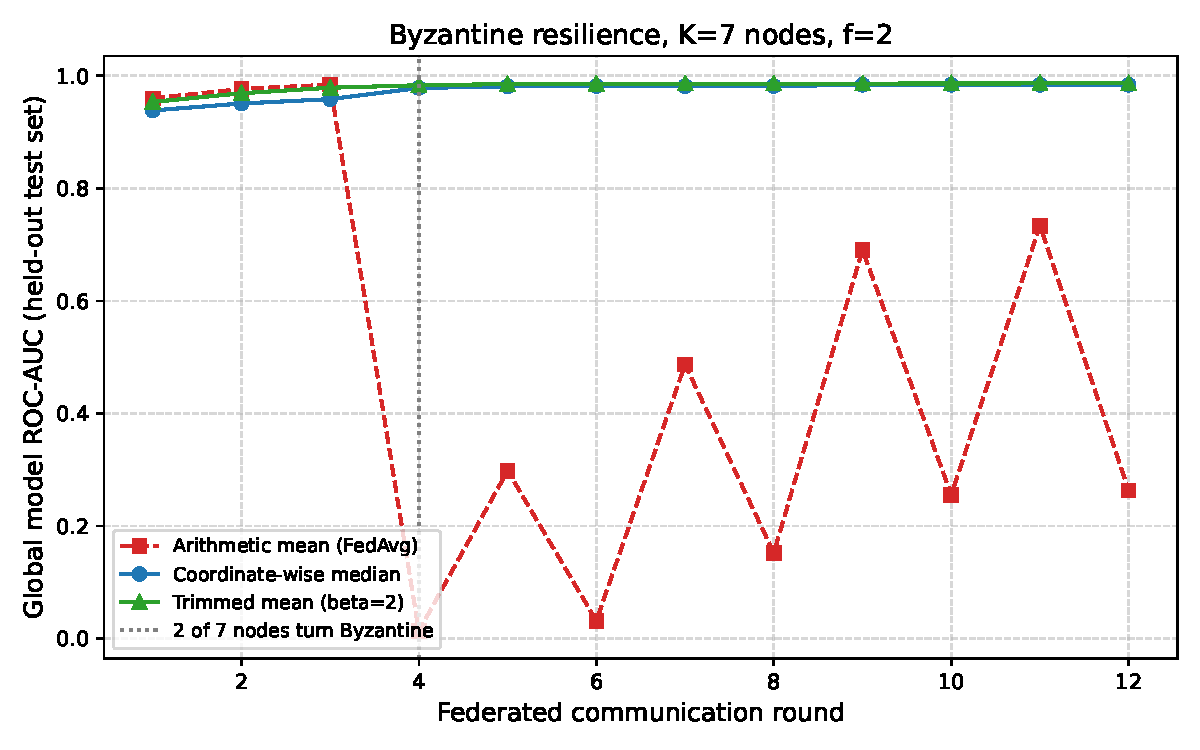
\includegraphics[width=0.95\columnwidth]{figures/poisoning_defense.pdf}
\caption{Bare-aggregator ablation, one seed (\texttt{poisoning\_experiment.py}, no norm gate): from round~4, two of seven nodes upload sign-flipped, $12\times$ amplified weights.}
\label{fig:eval-poison}
\end{figure}

\begin{table}[t]
\centering
\caption{Global-model ROC-AUC in the bare-aggregator ablation (\texttt{poisoning\_results.json}, one seed, no gate); the attack starts in round~4.}
\label{tab:eval-poison}
\begin{tabular}{@{}lccc@{}}
\toprule
\textbf{Aggregator} & \textbf{Round 3} & \textbf{Round 4} & \textbf{Round 12} \\ \midrule
Mean (FedAvg) & 0.984 & 0.014 & 0.263 \\
Coordinate median & 0.958 & 0.978 & 0.984 \\
Trimmed mean ($\beta{=}2$) & 0.979 & 0.983 & 0.986 \\ \bottomrule
\end{tabular}
\end{table}

Averaging falls from 0.984 to 0.014 in the first poisoned round, so the global model is inverted, and ends at 0.263. Median and trimmed mean keep improving, because the two poisoned uploads fall in the trimmed tails of every coordinate. This is the simplest attack in the study, and the deployed norm gate would reject it before aggregation (the next subsection shows exactly that), so Table~\ref{tab:eval-poison} says little about the shipped pipeline.

\subsubsection*{The deployed pipeline under five attacks}

\texttt{poisoning\_v2.py} imports the deployed \texttt{robust\_cloud.norm\_gate} ($\rho=4$) and \texttt{robust\_cloud.aggregate}, so gate and aggregation code are the shipped code. It runs $K\in\{10,20\}$ clients with Dirichlet ($\alpha=1$) non-IID mixes of web, API, SQLi and XSS data and log-normal client sizes, with production augmentation, for 10 rounds and 8 seeds. The malicious fraction goes up to 40\% ($f=4$ of 10; $f=8$ of 20). The attackers are omniscient and collude, and every client is assumed enrolled: authentication is out of scope, so $f$ is bounded by enrolment. The attacks are the $-12\times$ sign flip, ALIE of Baruch et al.\ (2019), a per-coordinate shift of the honest mean by $z$ honest standard deviations against its sign, with $z$ set from $K$ and $f$, the full-knowledge attack of Fang et al.~\cite{fang2020} on median and trimmed mean, label flipping at the clients, and a ``norm-bound'' attack that sends the reversed honest-mean direction scaled to 0.95 of the gate limit so that it passes. Each is run with each of mean, median and trimmed mean (trim~1 per side), with the gate on and off. The metrics are final-round ROC-AUC on held-out payloads, and TPR and FPR at the deployed $\tau=0.15$. The local trainer is a numpy SGD with its own hyper-parameters, not the scikit-learn recipe of the earlier sections, so absolute numbers differ from them.

\begin{table*}[t]
\centering
\caption{Poisoning with the deployed norm gate on (\texttt{poisoning\_v2\_results.json}; mean over eight seeds, final-round global model; FPR at $\tau=0.15$ on held-out payloads, median aggregator). The last row is the clean run ($f=0$) at the same $K$. Gate-off values are in Fig.~\ref{fig:eval-poison-v2}.}
\label{tab:eval-poison-v2}
\begin{tabular}{@{}lccccccccc@{}}
\toprule
 & \multicolumn{3}{c}{\textbf{K=10, f=2 (20\%)}} & \multicolumn{3}{c}{\textbf{K=10, f=4 (40\%)}} & \multicolumn{3}{c}{\textbf{K=20, f=8 (40\%)}} \\
\textbf{Attack} & mean & median & FPR & mean & median & FPR & mean & median & FPR \\ \midrule
Sign-flip & 0.967 & 0.964 & 0.03 & 0.966 & 0.962 & 0.05 & 0.969 & 0.968 & 0.02 \\
ALIE & 0.967 & 0.966 & 0.06 & 0.964 & 0.953 & 0.28 & 0.967 & 0.957 & 0.54 \\
Fang & 0.945 & 0.958 & 0.03 & 0.867 & 0.901 & 0.25 & 0.858 & 0.924 & 0.24 \\
Label-flip & 0.950 & 0.964 & 0.08 & 0.833 & 0.943 & 0.56 & 0.845 & 0.956 & 0.64 \\
Norm-bound & 0.173 & 0.963 & 0.06 & 0.117 & 0.942 & 0.51 & 0.091 & 0.951 & 0.67 \\ \midrule
None ($f{=}0$) & 0.968 & 0.965 & 0.02 & 0.968 & 0.965 & 0.02 & 0.969 & 0.968 & 0.04 \\ \bottomrule
\end{tabular}
\end{table*}

\begin{figure*}[t]
\centering
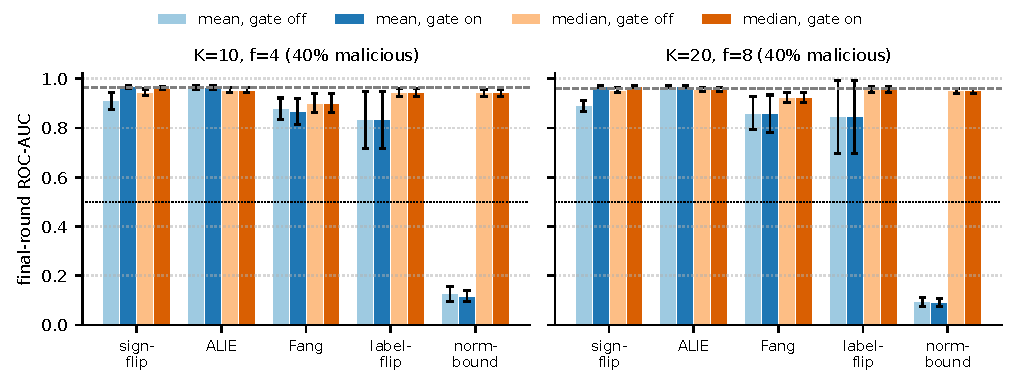
\includegraphics[width=0.85\textwidth]{figures/fig_poison_v2.pdf}
\caption{Final-round ROC-AUC by attack and aggregator, gate off and on, at 40\% malicious clients (left $K{=}10$, $f{=}4$; right $K{=}20$, $f{=}8$), mean $\pm$ 95\% interval over eight seeds (\texttt{poisoning\_v2\_results.json}). Dashed: pooled non-federated reference; dotted: AUC 0.5.}
\label{fig:eval-poison-v2}
\end{figure*}

The gate removes the one attack of the earlier experiment. At $K=10$, $f=2$ with the gate off, the mean aggregator ends at 0.602 $\pm$ 0.258 (its worst round is 0.052) and the trimmed mean (trim~1, which cannot cover two attackers) at 0.463; with the gate on both recover to 0.966 or higher, because the gate rejects every sign-flipped upload (rejection rate 1.00) and no honest one. The median is unaffected by this attack at 20\% malicious (0.963), but at 40\% ($K=10$) it needs the gate: 0.944 with an FPR of 0.49 without it, 0.962 with an FPR of 0.05 with it.

The gate does nothing against the other four attacks, which it rejects at rates of 0 to 0.04. The remaining damage depends on the aggregator and on the fraction, and is more visible in FPR than in AUC. At 20\% malicious the median with the gate stays within 0.958--0.966 AUC for all five attacks at $K=10$, with FPR at 0.15 between 0.03 and 0.08 (clean: 0.02); at $K=20$, $f=4$ the minimum is 0.961 and FPR 0.04--0.15 (clean: 0.04). At 40\% the picture is different. The median's AUC stays at 0.90--0.97, yet under every attack except the sign flip the FPR at $\tau=0.15$ is 0.24--0.67 (0.28 and 0.54 under ALIE at $K=10$ and $K=20$): a model that ranks well but, at the deployed threshold, blocks half the benign traffic. The mean collapses to AUC 0.09--0.17 under the norm-bound attack, which the gate cannot see by construction; the trimmed mean with trim~1 fails the same way at $f=4$ ($K=10$: 0.099) and at $K=20$, $f=4$ (0.886, FPR 1.00), since one trimmed value per side does not cover multiple attackers. No aggregator reaches the clean level under the Fang attack at 40\%, which is the attack designed against it: median 0.901 at $K=10$ and 0.924 at $K=20$.

Two limits qualify these results. First, the evidence concerns a simulation at $K\ge10$; the physical testbed has two gateways and thus $f=0$, where the median of two uploads is their mean (Section~\ref{sec:security}). Second, the AUC-FPR gap just described means that robust aggregation as configured preserves ranking at modest $f$ but not the deployed operating point at large $f$; re-calibrating $\tau$ after each aggregation round is untested.

\subsection{Edge Cost on ARM}
\label{sec:eval-hardware}

\emph{Provenance.} The measurements of this subsection come from the Raspberry~Pi~4 testbed (aarch64 Cortex-A72, 4\,GB; pure-Python gateway on port~8080 with a 15\,s synchronisation interval; load generator \texttt{stress\_test.py}) and are recorded only in the earlier draft \texttt{federated\_paper\_v5.tex}, not in a result file. They predate the final augmentation and the threshold change, which do not alter inference arithmetic. They must be re-measured and archived before the numbers are relied on.

For the 259-coefficient model, inference averages 0.229\,ms per scored string, a single-core ceiling of about 4{,}370\,strings/s, at a resident set of 10.4\,MB dominated by the interpreter. The gateway scores about four contexts per request (Section~\ref{sec:eval-deployed}), so the cost per request is of the order of four times that figure; this is arithmetic on two measurements, not a measurement. Under 1{,}000 requests at concurrency~10, repeated ten times, the threaded gateway sustained $452.5\pm24.3$\,req/s with median latency $20.5\pm0.7$\,ms and 95th percentile $32.2\pm2.5$\,ms and no failed request in 10{,}000. The HTTP stack, not the classifier, was the bottleneck: a single-threaded server serialised keep-alive connections and capped throughput at 42--56\,req/s until \texttt{ThreadingHTTPServer} replaced it. All requests were benign GETs answered with 200; throughput under mixed attack load and for 8\,KB bodies is unmeasured. ML-KEM-512 on the same board cost 0.122\,ms (key generation), 0.162\,ms (encapsulation) and 0.205\,ms (decapsulation) over 1{,}000 warmed-up trials. This is a component benchmark: the live \texttt{/update} and \texttt{/weights} endpoints do not use the derived key.

\subsection{Bandwidth and Data Sovereignty}
\label{sec:eval-bandwidth}

\begin{figure}[t]
\centering
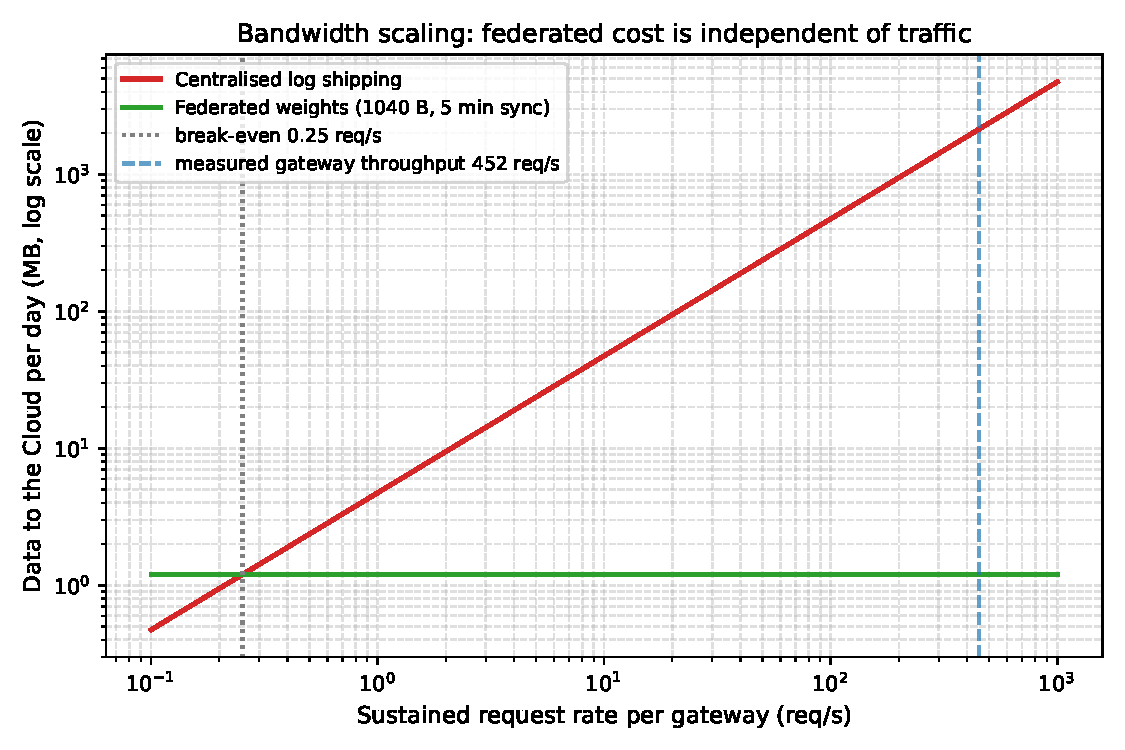
\includegraphics[width=0.95\columnwidth]{figures/fl_bandwidth.pdf}
\caption{Daily traffic to the cloud versus sustained request rate for two gateways (\texttt{bandwidth\_analysis.py}, analytic, 1{,}040\,B per update). The federated cost is flat because each synchronisation carries a fixed-size update.}
\label{fig:eval-bandwidth}
\end{figure}

Bandwidth comparisons commonly set a whole dataset against one update from one node. Here federation is charged for every round, node and direction. The 20-round training run transfers $20\times2\times2\times1{,}040=83{,}200$\,B against 332{,}983\,B of raw request payloads (mean 27.4\,B), a 75.0\% reduction (\texttt{bandwidth\_results.json}). In operation the costs scale differently: log shipping grows with traffic, federation with the synchronisation interval (Table~\ref{tab:eval-bandwidth}).

\begin{table}[t]
\centering
\caption{Daily cloud-bound traffic for two gateways, analytic, 1{,}040\,B per update (\texttt{bandwidth\_results.json}). The 99.94\% figure applies to the 300\,s interval; the deployed interval is 15\,s.}
\label{tab:eval-bandwidth}
\resizebox{\columnwidth}{!}{%
\begin{tabular}{@{}rrrrr@{}}
\toprule
\textbf{Rate} & \textbf{Sync} & \textbf{Centralised} & \textbf{Federated} & \textbf{Reduction} \\ \midrule
10\,req/s & 300\,s & 47.3\,MB & 1.2\,MB & 97.47\% \\
100\,req/s & 300\,s & 473.1\,MB & 1.2\,MB & 99.75\% \\
452\,req/s & 300\,s & 2{,}138.4\,MB & 1.2\,MB & 99.94\% \\
452\,req/s & 15\,s & 2{,}138.4\,MB & 24.0\,MB & 98.88\% \\ \bottomrule
\end{tabular}}
\end{table}

At the 15\,s interval of the testbed the reduction at 452\,req/s is 98.88\%. The break-even is about 0.25\,req/s per node at 300\,s, below which log shipping is cheaper. Three assumptions limit the comparison. The baseline ships every request's payload only (27.4\,B on average), omitting headers and metadata, but also omitting the sampled or flagged-only shipping a practical deployment would use. The update size is 1{,}040\,B (259 float32 values and a bias), whereas the implementation sends JSON text: the coefficient list in \texttt{fed\_model.json} serialises to 5{,}395\,B. With that size, which is arithmetic on the committed values and not a wire measurement, the 20-round training transfer would be 431{,}600\,B and exceed the raw payloads it replaces by 30\%, and the 15\,s reduction at 452\,req/s would be 94.2\%. And none of the figures covers retransmission, TLS or a post-quantum handshake, which are not in the live path. Federation keeps request content inside the site boundary, which Industrial Data Space governance requires; the bandwidth saving is secondary and depends on the update encoding.

\subsection{Unresolved Limits of the Evidence}
\label{sec:eval-limits}

\paragraph{Benign data.}
Every benign string outside CSIC is a path token or a generated string; no captured traffic from a working site is used. The CSIC result shows that the scorer, not just its threshold, fails on an external benign set, so the false-positive figures of Tables~\ref{tab:eval-detection} and~\ref{tab:eval-deployed} should be read as lower bounds.

\paragraph{Operating point.}
The deployed threshold was set on the shipped model and tested here only on retrained models. The shipped model's own held-out behaviour at $\tau=0.15$ has no estimate that is free of training overlap; the CSIC and synthetic-probe results are the only evidence about it, and both are adverse.

\paragraph{Federation gain.}
The advantage of federation over the best silo is below one standard deviation in the exact-unique studies and negative against the test-oracle silo in the cluster split; against pooled training it is nil. What remains is protection against the silo trained on the wrong benign domain and a lower false-positive rate at the deployed threshold than either silo, but a higher one than pooling.

\paragraph{Scale and attacks.}
The detection experiments use $K=2$ nodes with attack data drawn from one shared pool in the domain axis. The poisoning study reaches $K=20$ in simulation with an omniscient, fixed-strategy adversary; there are no adaptive input-space evasions of the linear model, no backdoors, and a physical $f=0$. Attack classes are limited to SQLi and XSS strings from fuzzing lists with 681 and 523 unique entries, so per-seed recall has a standard deviation of 0.06 at 0.1\% FPR.

The security consequences of the update path itself, which these experiments assume and do not exercise, are the subject of Section~\ref{sec:security}.
\emergencystretch=0pt
